\chapter{Lecture 2}
\lhead{January 14, 2015}
\chead{21-366 Lambda Calculus Lecture 2}

\section{Construction Trees}
\index{Construction Tree|textbf}
During the previous lecture, we proved that proper pairings of parenthesis are unique, and that each term has a proper pairing. We also observed that each term has an associated construction tree. From this we can demonstrate that construction trees are unique.\\

\subsection{Generating Construction Trees}
It is nice to know that unique construction tree representations exist for terms, but it would be useful sometimes to know what those construction trees actually are. We can describe an algorithm that, when given a term, provides the construction tree for that term.\\

\margnot{Note}{ Even though we omit parens sometimes when writing terms, when we prove statements involving parenthesis, we treat the terms as if no parens have been omitted.}

In the most simple case, a term with no parens is a variable. Variables are terminal nodes in our construction tree. If there are parenthesis, then we begin with the leftmost left parent. Since the pairing is proper, this leftmost paren must be paired with the rightmost right paren. Otherwise, a crossing would have occurred. We then have one of three cases: either the first symbol is a variable, the first symbol is a left paren, or the first symbol is a \l. If the first symbol is a variable, then our term is of the form $(xY)$, and has this construction tree:

\begin{center}
  \begin{tikzpicture}[grow'=up]
    \Tree[.$(xY)$ [.$x$ ] [.$Y$ ] ]
  \end{tikzpicture}
\end{center}

$x$ is terminal, so we induct on $Y$. Otherwise, if the next symbol is a left paren, we have a term of the form $((X)(Y))$. We can then induct on both $X$ and $Y$ with the following construction tree:

\begin{center}
  \begin{tikzpicture}[grow'=up]
    \Tree[.$(XY)$ [.$X$ ] [.$Y$ ] ]
  \end{tikzpicture}
\end{center}

In our final case, we have that our term is of the form $(\l xX)$, which has the construction tree:

\begin{center}
  \begin{tikzpicture}[grow'=up]
    \Tree[.$(\l xX)$ [.$(X)$ ] ]
  \end{tikzpicture}
\end{center}

Again, we induct on $X$. From this we can generate a construction tree for any term.\\

\examplebox{Example: Construction Tree for $(\l x(X(xy)))$}{
  We begin by using the rule for constructing a tree from a lambda term:
  \begin{center}
    \begin{tikzpicture}[grow'=up]
      \Tree[.$(\l x(X(xy)))$ [.$((X)(xy))$ ] ]
    \end{tikzpicture}
  \end{center}
  We then use the rule for application terms:
  \begin{center}
    \begin{tikzpicture}[grow'=up]
      \Tree[.$(\l x(X(xy)))$ [.$((X)(xy))$ [.$(X)$ ] [.$(xy)$ ] ] ]
    \end{tikzpicture}
  \end{center}
  Finally, we treat the $X$ path as completed, since we havedn't defined what $X$ is, and use the application rule once more on the $(xy)$ path:
  \begin{center}
    \begin{tikzpicture}[grow'=up]
      \Tree[.$(\l x(X(xy)))$ [.$((X)(xy))$ [.$(X)$ ] [.$(xy)$ [.$x$ ] [.$y$ ] ] ] ]
    \end{tikzpicture}
  \end{center}
}



\section{Some Definitions}
It is somewhat cumbersome to always have to write ``a term of the form $(XY)$'' when we want to talk about subtermsof an application. When we have a term of the form $(XY)$, we say that $X$ is in \textbf{function position}\index{Function Position}, and $Y$ is in \textbf{argument position}\index{Argument Position}. We also say that $Y$ is applied to $X$.\\

\subsection{Subterms}
\index{Subterm|textbf}
Let $Y$ be a term. $Y$ is a subterm of $X$ if $Y$ is also a substring of $X$, with the exception of a variable following a \l.\\

\noindent\textbf{Trichotomy Law: }\index{Trichotomy Law} Given any two subterm occurances\footnote{In this course, subterm occurances will be notated with primes.} $Y',Z'$ of a term $X$, then either they are disjoint or one contains the other.\\

\subsection{Free and Bound Variables}
\index{Free Variable|textbf}\index{Bound Variable|textbf}
In a lambda term $(\l x.X)$, we say that the variable $x$ is \textbf{bound} by the term, because the contents of the term will be determined by the argument provided to the lambda. Variables which are not bound in this way are called \textbf{free.} It is possible for variables to be free in one term, but bound by a term which occurs higher in the construction tree. It should be clear, for example, that the term $x$ has one free variable: $x$ itself. However in the term $\l x.X$, it is bound by the lambda.\\

So, what happens to bound and free variables when we have a term of the form $(XY)$? Since there are no lambdas introduced, the status of the variables cannot change. The variables which were bound remain bound, and the variables which are free remain free. We can summarize the rules for determining which variables are bound and which are free as follows:\\

\examplebox{Summary of Bound and Free Variables}{
\begin{eqnarray*}
  FV(x) &=& \{x\}\\
  BV(x) &=& \emptyset\\
  FV((XY)) &=& FV(X) \cup FV(Y)\\
  BV((XY)) &=& BV(X) \cup BV(Y)\\
  FV((\l xX)) &=& FV(X) - \{x\}\\
  BV((\l xX)) &=& BV(X) \cup \{x\}\\
\end{eqnarray*}
}

It is useful when attempting to determine which variables of a term are bound and which are free by hand, to draw the construction tree for the term. It is obvious what variables in the roots of the tree are bound, and which are free. From there, the recursive definitions given above can be employed.\\

\examplebox{Example: Determining the Bound Variables of a Term}{
  Say that we have a term $((xx)(\l x.(xx)))$ for which we want to determine the free variables. We begin by drawing the construction tree:
  \begin{center}
    \begin{tikzpicture}[grow'=up]
      \Tree[.$((xx)(\l x.(xx)))$ [.$(xx)$ [.$x$ ] [.$x$ ] ] [.$(\l x.(xx))$ [.$(xx)$ [.$x$ ] [.$x$ ] ] ] ]
    \end{tikzpicture}
  \end{center}
  All of the root nodes of the tree are terms $x$, which have free variables $x$. Both terms of $(xx)$ are of the form $(XY)$, so their free variables are the union of the free variables of their subtrees, or $x$. The lambda term $\l x.xx$ binds $x$, so $x$ is no longer free. The top term inherits the free and bound variables of its subtrees once more, so the bound variables are $x$, and the free variables are... $x$.
}

The example above illustrates a subtlety which is easy to miss. The variable $x$ in the left subtree is not the same as the variable $x$ in the right subtree. We wrote them as the same symbol, but in actuality they are wholly unrelated. If we represent the $x$s in the left subtree as $y$s instead, the situation makes itself clear.

\begin{center}
  \begin{tikzpicture}[grow'=up]
    \Tree[.$((yy)(\l x.(xx)))$ [.$(yy)$ [.$y$ ] [.$y$ ] ] [.$(\l x.(xx))$ [.$(xx)$ [.$x$ ] [.$x$ ] ] ] ]
  \end{tikzpicture}
\end{center}

The free variables are $y$, and the bound variables are $x$.

\section{Minimizing Parenthesization}
\margnot{Jan \L usckasevicz}{ Jan was born in 1878 in Poland. He worked in analytical philosophy and logic. He is best known for Polish notation.}
We've talked a bit so far about ways to reduce the number of parenthesis needed to unambiguously determine the construction tree of a term. Now we will formally introduce three strategies for removing parenthesis: Polish notation, Church's dot notation, and left associative deletion.

\subsection{Polish Notation}
\index{Polish Notation}


\margnot{Polish Notation}{ Polish notation is sometimes referred to in other contexts as ``prefix notation.'' Equivalently, there is a ``postfix notation'' which is sometimes called Reverse Polish Notation.}

Polish notation was invented by Jan \L uckasevicz\index{Lusckasevicz, Jan@\L usckasevicz, Jan} in 1924. We use only the symbols $\l$ and $($, plus variables $x,y,z$ and terms $X,Y$. The key feature of Polish notation is that operators are placed before their arguments. Take, for example, the expression $3 + 4$. The operator in this expression, the $+$ occurs between the arguments, $3,4$. In Polish notation, we would instead write $+ 3 4$. In this simple case it is not immediately obvious what is gained by this. When we try it on a larger expression, it becomes clear what the advantage is:
\begin{equation*}
  ((3 + 4) \times (2 + 2)) / (1 + 5) \Rightarrow / \times + 3\ 4 + 2\ 2 + 1\ 5
\end{equation*}
Notice how by rearranging the expression, we can remain unambiguous without parenthesis. We can adopt a similar style for writing lambda terms. We use the terms $\l,(, x, y, z$ where $x, y, z$ are variables, and $X,Y$ are terms.\\

\examplebox{Example: Lambda Terms in Polish Notation}{
  \begin{eqnarray*}
    (XY\\
    \l xX
  \end{eqnarray*}
}

We can notice that terms written using Polish notation can be fairly straightforwardly derived from terms which do not, simply by omitting the right parens. Although this does significantly reduce the number of necessary parenthesis, it also makes the terms much more difficult to read, so we will not actually use this method in practice.

\subsection{Church's Dot Notation}
\index{Church, Alonzo!Church's Dot Notation|textbf}
\margnotTwo{Willard Van Orman}{Quine}{ Born in 1908, the American philsopher and logic Quine spent his life at Harvard University.}

Another convention we can use is a dot notation developed by Quine\index{Quine, Willard Van Orman}, called Church's dot notation. Using this notation, we take a term with some number of initial lambdas, and remove the parens around all of them, placing a dot after the last one. So if we have an expression of the form
\begin{equation*}
  (\l x_1(\l x_2(\l x_3\ldots(\l x_nX)\ldots)))
\end{equation*}
We can write it as
\begin{equation*}
  (\l x_1x_2\ldots x_n.X)
\end{equation*}
This makes it much easier to write out functions which take in multiple arguments as lambda terms. It is worth mentioning currying again here. Writing a curried function in dot notation might make it seem like we are again working with functions which take in multiple arguments again. We are not.

\examplebox{Example: Dot Notation Representation of $S$}{
  \begin{equation*}
    S := (\l x (\l y (\l z((xy)(yz))))) = \l xyz.((xy)(yz))
  \end{equation*}
}

\subsection{Left Association}
\index{Left Association|textbf}
We can delete all of the parenthesis around applications where the subterm is not in argument position. So in a term $(XY)$, we can delete parens around $X$, if any occur. We also retain the outermost set of parenthesis in a formal sense, although we will tend to omit them in practice. So if $X = (UV)$ and we have a term $((UV)Y)$ we would delte the parenthesis around $(UV)$ to get $(UVY)$.

\examplebox{Example: Left Association Representation of $S$}{
  \begin{equation*}
    S := (\l x (\l y (\l z((xy)(yz))))) = (\l x (\l y (\l z(xy(yz)))))
  \end{equation*}
}

It is not immediately obvious that this strategy for deleting parenthesis preserves uniqueness. This is proven in the next lecture.

\section{Proper Extensions}
\index{Proper Extension|textbf}
We say that a string $s_1$ is a proper extension of some string $s_2$ if $s_1$ can be written as the concatenation of $s_2$ and another nonempty string. The string ``Hello world'' is therefore a proper extension of the string ``Hello'' by the concatenation of the extra string `` world''. We claim that no term is a proper extension of another term as a string read from left to right.\\

We can prove this by induction on the sum of the lengths of the two sequences. The smallest sequence is a variable $x$. No term can be an extension of a variable because a left paren is necessary. Now consider a term $X$ with an extension $Y$. There are two possible cases: either $X$ is of the form $X = \l uU$ or $X = (UV)$.\\

If $X = \l uU$, then the only way to extend $X$ is if $Y$ begins with $\l u$, which can only be extended into a term of the form $\l uV$. Since we claim by our induction hypothesis that $V$ is not a proper extension of $U$ for ally $U$, $V$ smaller than $X$,$Y$, and $U$ must necessarily be an extension of $U$, we have a contradiction.\\

In our other case, we have that $X = (UV$. Therefore $Y$ must begin with a paren, and so be of the form $Y = (ZW$. This implies that $ZW$ is an extension of $UV$. By our induction hypothesis, $U = Z$ and $V = W$, so there can be no extension. So construction trees are unique.